
\begin{figure}[tb]
	\centering
	\makebox[\textwidth]{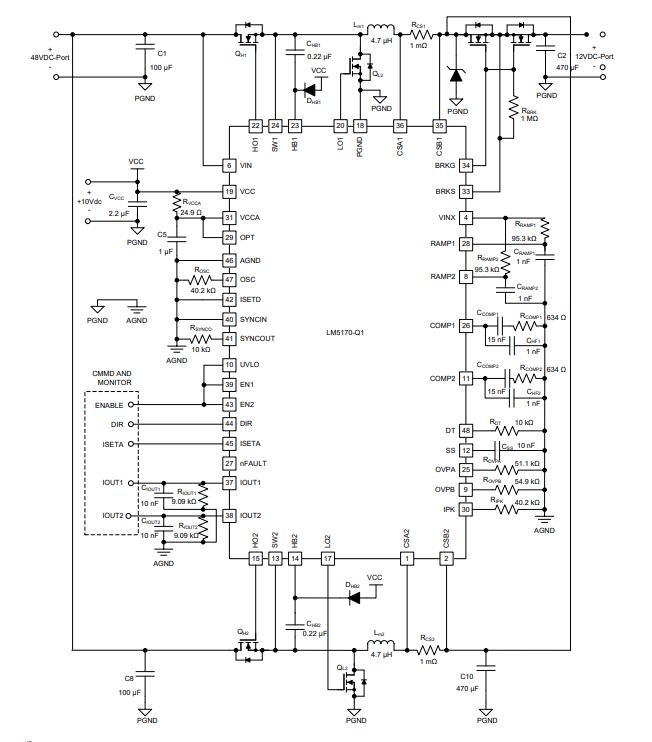
\includegraphics[width=0.7\paperwidth]{Chap_Miselleneous/Chap04_Mise/Figures/LM5170_Typical_ciruit.PNG}}
    \caption{Typical Bidirectional circuit of the LM5170}
    \label{fig:Typical Bidirectional circuit of the LM5170}
\end{figure}

\begin{figure}[tb]
	\centering
	\makebox[\textwidth]{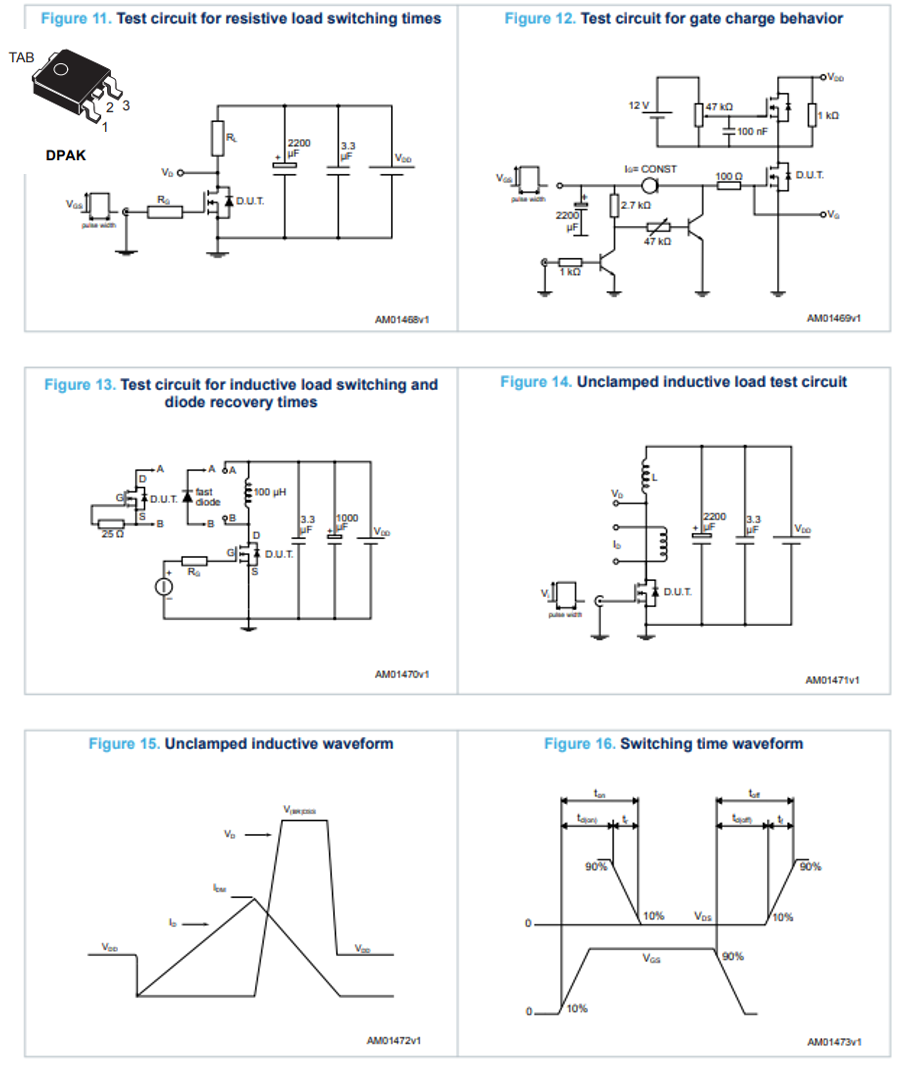
\includegraphics[width=0.8\paperwidth]{Chap_Miselleneous/Chap04_Mise/Figures/Switch_FET.PNG}}
    \caption{STD20NF06L Application typical circuit and package}
    \label{fig:STD20NF06L Application typical circuit and package}
\end{figure}

\begin{figure}[tb]
	\centering
	\makebox[\textwidth]{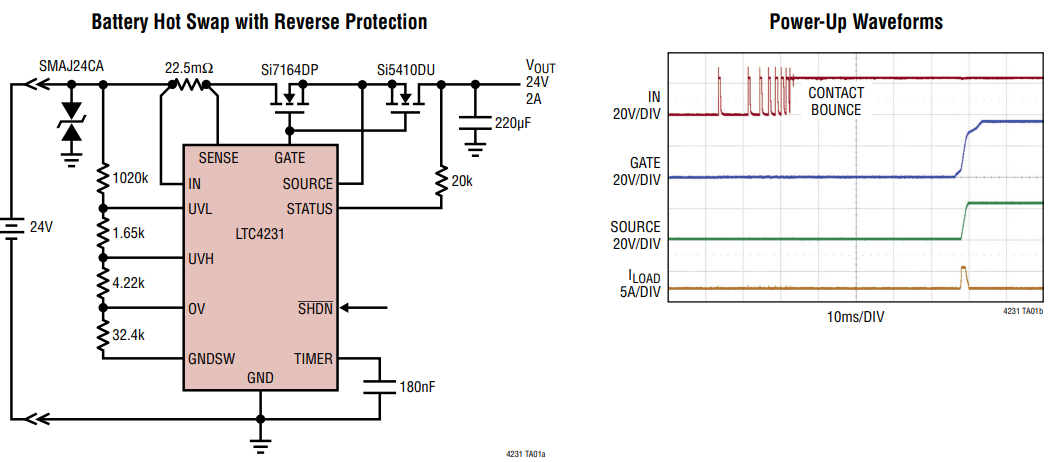
\includegraphics[width=0.7\paperwidth]{Chap_Miselleneous/Chap04_Mise/Figures/LTC4231.PNG}}
    \caption{LTC4231 Application circuit and the Operational waveform }
    \label{fig: LTC4231 Application circuit and the Operational waveform }
\end{figure}

\subsubsection{ Design Example for the LTC4321 Gate Driver :}
As Design takes the following specifications for the Figure\ref{fig: LTC4231 Application circuit and the Operational waveform } application circuit. The application is rated for a max battery pack voltage of 24V at 5A, $C_L=100\mu F$. UV raising=23V, UV falling = 22V, OV rising = 26V.

Sense Resistor :\\
\begin{equation}\label{eq:LTC_Rsense}
	R_{sense}  = \frac{\Delta V_{sense(CB)(MIN)}}{I_{Inrush}} = \frac{\left(47mV \right)}{\left(2A\right)} = \left(23.5m \Omega\right)
\end{equation}
Use RSENSE = 22.5mΩ for margin. Worst case analog current limit:\\
\begin{equation}\label{eq:LTC_Ilimit_min}
	I_{LIMIT(MIN)} = \frac{\Delta V_{sense(ACL)(MIN)}}{R_{sense}} = \frac{\left(65mV \right)}{\left(23.5m \Omega \right)} = \left(2.89A\right)
\end{equation}
\begin{equation}\label{eq:LTC_Ilimit_max}
	I_{LIMIT(MAX)} = \frac{\Delta V_{sense(ACL)(MAX)}}{R_{sense}} = \frac{\left(90mV \right)}{\left(23.5m \Omega \right)} = \left(4A\right)
\end{equation}
Calculate the worst-case time it takes to charge up CL analog current limit:\\
\begin{equation}\label{eq:LTC_Tcharge_max}
	t_{CHARGE(MAX)} = \frac{ C_{L}\times V_{IN}}{I_{LIMIT(MIN)}} = \frac{\left(100\mu F \times 24V \right)}{\left(2.89A \right)} = \left(0.9ms\right)
\end{equation}
For inrush control using analog current limit, $t_{CHARGE(MAX)}$ must be less than the circuit breaker delay (tCB) for a proper start-up \cite{LTC4231_User_Datasheet}.

The worst-case power dissipation in MOSFET M1 occurs "\\
\begin{equation}\label{eq:LTC_Pdissp}
	P_{DISS} = V_{IN} \times I_{LIMIT(MAX)}  = \left(24V \times 4A\right) = \left(96W\right)
\end{equation}

during a severe overcurrent fault when the current is controlled by analog current limit for the duration of tCB:
\begin{equation}\label{eq:LTC_Ct}
    C_{T} = \frac{ t_{Cb}}{24V} = \frac{\left(2mS \right)}{\left(24V \right)} = \left(82nF\right)
\end{equation}

If a low inrush current ($< \Delta V_{SENSE(CB)}$) is preferred, refer
to the Figure \ref{fig: LTC4231 Application circuit and the Operational waveform } application circuit which uses a gate capacitor CG to limit the inrush current. Choose IINRUSH = 0.5A
which is set using $C_G$ \cite{LTC4231_User_Datasheet}:

\begin{equation}\label{eq:LTC_Cg}
	C_{G} = \frac{ C_{l}\times 10\mu A}{I_{Inrush}} = \frac{\left(100\mu F \times 10\mu A \right)}{\left(2.89A \right)} = \left(20nF\right)
\end{equation}
The time to charge up CL with 0.5A is:
\begin{equation}\label{eq:LTC_Tcharge}
    t_{CHARGE(MAX)} = \frac{ C_{L}\times V_{IN}}{I_{Inrush}} = \frac{\left(100\mu F \times 24V \right)}{\left(0.5A \right)} = \left(48ms\right)
\end{equation}
The average power dissipation in the MOSFET M1 during this start-up is:
\begin{equation}\label{eq:LTC_Pdissp_average}
    P_{DISS} = V_{IN} \times I_{LIMIT(MAX)}  = \left(24V \times 0.5A\right) = \left(6W\right)
\end{equation}

\begin{figure}[h]
	\centering
	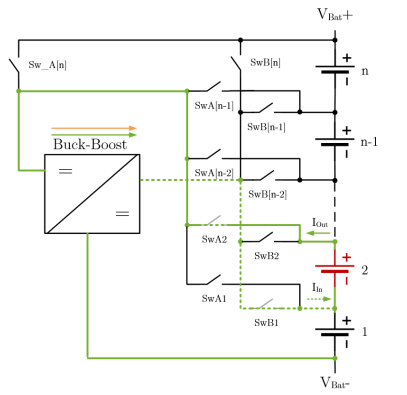
\includegraphics[width=0.4\textwidth]{Chap04/Figures/Type2a_ABMS.PNG}
	\caption{\textit{Type Ib} Active Balancing Circuit} 
	\label{fig:Type1b Active Balancing Circuit }
\end{figure}

\begin{figure}[h]
	\centering
	\subfigure[Single operation bidirectional buck-boost converter (Low-side)]{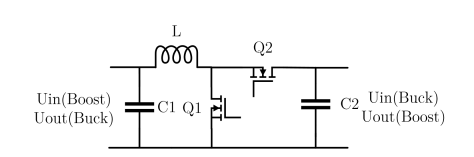
\includegraphics[scale=.5]{Chap_Miselleneous/Chap04_Mise/Figures/Bi_buck_boost_low_side.PNG}}
	\qquad
	\subfigure[ Single operation bidirectional buck-boost converter (High-side)]{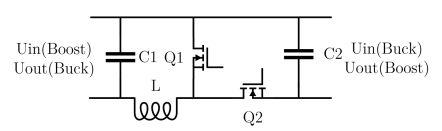
\includegraphics[scale=.5]{Chap_Miselleneous/Chap04_Mise/Figures/Bi_buck_boost_High_side.PNG}}
	\caption{Typical Schematics of the Low side and High Side buck-boost Converter}
	\label{fig:Typical Schematics of the Low side and High Side buck boost Converter}
\end{figure}